%Feedback:
%A major challenge is how to simplify the gameplay so that starting the
%game is immediately a fun and funny experience. A core concept of the
%game is to parody a serious topic and use stereotypical things like
%praying and books in a humorous way. The gameplay should also support
%this effort, so that it is fun and funny, rather than serious and
%difficult. I would consider how to make the game work with only one or
%two players by including some simple AI concepts that fit this
%framework. For example, many AI players can be forming groups and
%casting wonders, but without much smarts or effectiveness. It's up to
%the human players to focus the efforts of the group in a strategic
%way.
%=================
%Summarized:
% - instant fun
% - game should work with 1,2 players
% - AI required

{\documentclass[11pt,a4paper,titlepage,table]{article}
\usepackage[a4paper]{geometry}
\usepackage[utf8]{inputenc}
\usepackage[english]{babel}
\usepackage{lipsum}



\usepackage{amsmath, amssymb, amsfonts, amsthm, fouriernc}
% mathtools for: Aboxed (put box on last equation in align envirenment)
\usepackage{microtype} %improves the spacing between words and letters

\usepackage{graphicx}
\graphicspath{ {./pics/} {./eps/}}
\usepackage{epsfig}
\usepackage{epstopdf}
\usepackage{colortbl}


%%%%%%%%%%%%%%%%%%%%%%%%%%%%%%%%%%%%%%%%%%%%%%%%%%
%% COLOR DEFINITIONS
%%%%%%%%%%%%%%%%%%%%%%%%%%%%%%%%%%%%%%%%%%%%%%%%%% 
\usepackage{colortbl}
\usepackage[usenames,dvipsnames,svgnames,table]{xcolor}
\usepackage{float}
%%%%%%%%%%%%%%%%%%%%%%%%%%%%%%%%%%%%%%%%%%%%%%%%%%
\definecolor{MyColor1}{HTML}{75A42E}
\definecolor{MyColor2}{HTML}{75A42E}
\definecolor{MyColor3}{HTML}{4D6D1E}
\definecolor{green1}{HTML}{EAF5DB}
\definecolor{green2}{HTML}{C2E193}
\definecolor{maroon}{cmyk}{0,0.87,0.68,0.32}
\newcommand{\textb}{\color{Black} \usefont{OT1}{lmss}{m}{n}}
\newcommand{\blue}{\color{MyColor1} \usefont{OT1}{lmss}{m}{n}}
\newcommand{\blueb}{\color{MyColor1} \usefont{OT1}{lmss}{b}{n}}
\newcommand{\red}{\color{LightCoral} \usefont{OT1}{lmss}{m}{n}}
\newcommand{\green}{\color{Turquoise} \usefont{OT1}{lmss}{m}{n}}
%%%%%%%%%%%%%%%%%%%%%%%%%%%%%%%%%%%%%%%%%%%%%%%%%%




%%%%%%%%%%%%%%%%%%%%%%%%%%%%%%%%%%%%%%%%%%%%%%%%%%
%% FONTS AND COLORS
%%%%%%%%%%%%%%%%%%%%%%%%%%%%%%%%%%%%%%%%%%%%%%%%%%
%    SECTIONS
%%%%%%%%%%%%%%%%%%%%%%%%%%%%%%%%%%%%%%%%%%%%%%%%%%
\usepackage{titlesec}
\usepackage{sectsty}
%%%%%%%%%%%%%%%%%%%%%%%%
%set section/subsections HEADINGS font and color
\sectionfont{\color{MyColor1}}  % sets colour of sections
\subsectionfont{\color{MyColor2}}  % sets colour of sections
\subsubsectionfont{\color{MyColor3}}  % sets colour of sections


%set section enumerator to arabic number (see footnotes markings alternatives)
\renewcommand\thesection{\arabic{section}.} %define sections numbering
\renewcommand\thesubsection{\thesection\arabic{subsection}} %subsec.num.

%define new section style
\newcommand{\mysection}{
	\titleformat{\section} [runin] {\usefont{OT1}{lmss}{b}{n}\color{MyColor1}} 
	{\thesection} {3pt} {} } 

%%%%%%%%%%%%%%%%%%%%%%%%%%%%%%%%%%%%%%%%%%%%%%%%%%
%		CAPTIONS
%%%%%%%%%%%%%%%%%%%%%%%%%%%%%%%%%%%%%%%%%%%%%%%%%%
\usepackage{caption}
\usepackage{subcaption}
%%%%%%%%%%%%%%%%%%%%%%%%
\captionsetup[figure]{labelfont={color=MyColor1}}


\makeatletter
\let\reftagform@=\tagform@
\def\tagform@#1{\maketag@@@{(\ignorespaces\textcolor{red}{#1}\unskip\@@italiccorr)}}
\renewcommand{\eqref}[1]{\textup{\reftagform@{\ref{#1}}}}
\makeatother
\usepackage{hyperref}
\hypersetup{colorlinks=true}

%%%%%%%%%%%%%%%%%%%%%%%%%%%%%%%%%%%%%%%%%%%%%%%%%%
%% PREPARE TITLE
%%%%%%%%%%%%%%%%%%%%%%%%%%%%%%%%%%%%%%%%%%%%%%%%%%
\title{\blue  
	\begin{figure}[h!]
  		\centering
    	\includegraphics[width=1\textwidth]{img/logoDraft2}
	\end{figure}
	\blueb Battle of Origins | Theory Defender}
\author{}
\date{\today}
%%%%%%%%%%%%%%%%%%%%%%%%%%%%%%%%%%%%%%%%%%%%%%%%%%



\begin{document}
	\maketitle
	\hypersetup{linkcolor=MyColor1}
	
	\begin{figure}[h!]
  		\caption{Battle of Origins | Theory Defender}
  		\centering
    	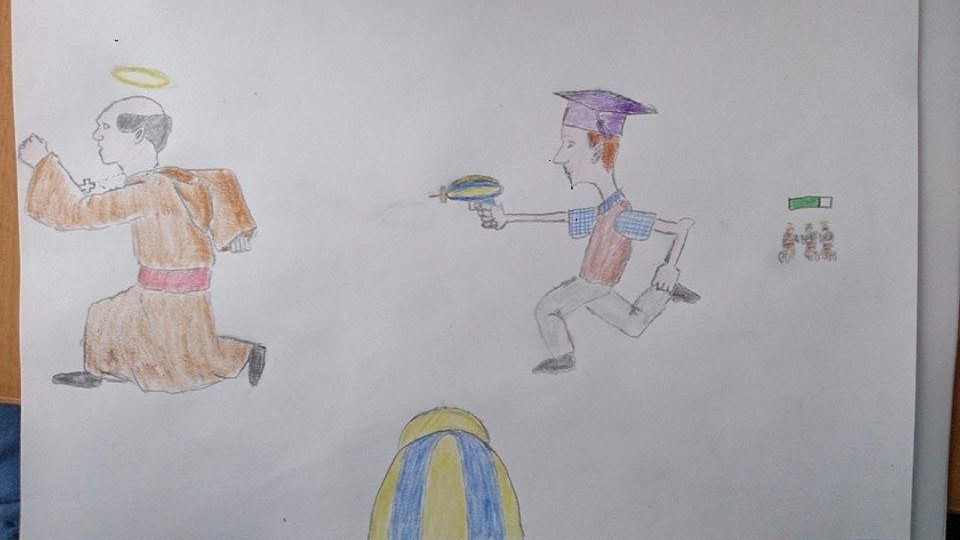
\includegraphics[width=1\textwidth]{img/FPSPerspective}
	\end{figure}	
	
	\tableofcontents
	\section{Game Description}{
		%–	 1 to 3 pages detailed description
		%–	3 pages sketches / sample images 
		%–	Highlight and justify design choices 

		\subsection{Storyline}{
			We live in a world where to all questions humanity asks itself an answer is found in religion and science. Two branches that split the world into two parties drifting more and more apart. Neither of them willing to accept or even listen the opinion of the other. But humanity cannot progress when it is at conflict with itself. The time has come to reunite the population of our planet and to lead humanity on its one and only true path. For a peaceful and strong world one side needs to disappear forever. Starting with the most fundamental question: "how did we become what we are today?". Was it an instant creation of perfection or an evolution that took billions of years to make us who and how we are to this day. Choose your belief and convert everyone who dares to challenge your norm of existence in the epic "\textit{Battle of Origins}". 
		}\label{sub:sub1}


		\subsection{Gameplay}{
	
			Before the match begins the player may choose a belief. Either religionist or evolutionist. The main aim of the game is to convert the entire opposing team to your belief. \\
			The teams will consist of 30 people each. Non-human players will be controlled by an artificial intelligence. Each player is able to blast the players of the other team away, causing them to fly through the air and temporarily take their ability to move. To convert the opposing player to your belief a big wonder must be cast. A big wonder can be generated by standing together as a group from the same team. Standing together allows the player to press the pray/study button which will start filling the big wonder progress bar. While standing together the players have an increased vulnerability. Meaning if an opposing player A is shooting at a player B who is currently praying/studying, player B will be hurled further away than he would have been if he had not been studying/praying. In addition while the players are standing together the rest of the map is blurred out so they cannot see approaching enemies. This can only be done if we use multiple screens. When releasing the pray/study button the player has a cool-down of 2 seconds before he can start running and shooting again. The speed of the wonder-creation progress is determined by two factors:
			\begin{enumerate}
				\item \textbf{The size of the group:}\\
							The more people close to each other, the quicker the progress bar will increase
				\item \textbf{Wonder Skill:}\\
				The creating-wonder skill of each player that is currently in the group (see subsection \ref{sec:evolvingUpgrades})
			\end{enumerate}
			Once a big wonder is generated it is indicated by multiple representations:
			\begin{itemize}
				\item The progress bar is full (visible to all players)
				\item One player is now in possession of the big wonder (see subsection \ref{sec:visual_diff} to see visual representation)
				\item A sound lets all players know that a big wonder is ready
			\end{itemize}
			The player who is in possession of the big wonder can now cast this whenever he wishes. While he is in possession he cannot be converted by a big wonder of the other team. Furthermore the possessing player has an increased running speed. A timer lets all players know how much time there is left before the wonder cannot be cast anymore. Once the big wonder is cast, the player becomes immune to all types of attacks (main attacks and big wonder conversion) and he is able to control the big wonder's area of effect. Any opposing player who is in the area of effect will be converted to the own team. While the wonder is active the progress bar decreases. Once it has reached zero the wonder will be deactivated and the player will have normal running speed and be vulnerable to all attacks again. Players of the same team can remain studying/praying while the wonder is active in order to lengthen the period of the wonder.
			
		\subsection{"Death" of players}
			There is no real death in the game. One can only hurl the other players through the field and making the unable to move for a period of time. There are two modes that control what happens after a player is converted. This mode can be selected by the player at the beginning of the game:
			\begin{itemize}
				\item[mode 1:] If a user-controlled player is converted he takes control of another computer controlled player of the team he originally picked, as long as there still exists one. If no computer controlled player is left in the team the player enters spectator-mode until computer controlled players are available again. This simply allows him to watch the game without having any influence.
				\item[mode 2:] If a user-controlled player is converted the user remains in control of the player but is now helping the other team to convert his originally selected team. This results in all players to be winners in the end.
			\end{itemize}
			
		}\label{sub:sub2}%

		
		

		
		
		\subsection{Evolving Upgrades }{
			Players will evolve on the fly while playing. They will not have the ability to choose an upgrade themselves. The more they perform a specific action, the better they will become at it. Following is a list of automatically evolving skills:
			\begin{itemize}
				\item Running Speed
				\item Power of main attack
				\item Precision of main attack
				\item Contribution to creating a big wonder
				\item Immunity against attacks
				\end{itemize}
			The visual difference of each upgrade can be seen in subsection \ref{sec:visual_diff}. Each player starts with 0-skill points on each skill. A class can be chosen before the game starts. Choosing a class will give an initial boost in a certain skill or allow the player to gain skill points in a certain skill faster.
		}\label{sec:evolvingUpgrades}
		
		
		\subsection{Visual Difference}{
			Although each player has the same power and tools, they are visually and audibly different depending on the chosen belief. Here is a table of what each part will look like
			\subsubsection{Main Game Aspects}{ 
				See table \ref{table:main}
				\begin{table}[h!]\centering
					\begin{tabular}{r!{\color{green2}\vrule}l!{\color{green2}\vrule}p{5cm}l!}
1						& \textbf{Religious} & \textbf{Evolutionist} \\
						\rowcolor{green1}
						\textit{Main Weapon} & Force push &	Blast gun \\
						\textit{Main Weapon  (upgrade)} &	Super force push &	Blast cannon \\
						\rowcolor{green1}
						\textit{Main attack}&	Use force push &	Shoot blast gun/cannon  \\
						\textit{Big Wonder} & Rays of god &	Rain of books \\
						\rowcolor{green1}
						\textit{ Creating Big Wonder} &	Praying&	Studying \\
						\textit{Big Wonder finished creating sound} & Angels singing "\textit{Aaaaah}" &	Pen on paper scribbling OR Voice saying "\textit{Q.E.D}" \\
						\rowcolor{green1}
						\textit{ Possessing wonder} &	Wings &	Carrying big book, Big glasses, robot, orbiting planets/atoms OR light bulb above head\\			
					\end{tabular}
				\caption{\textit{Main Game Aspects}}
				\label{table:main}
				\end{table}	
					
\begin{figure}[ht]
\centering
\begin{minipage}[t]{0.4\textwidth}
	\centering
	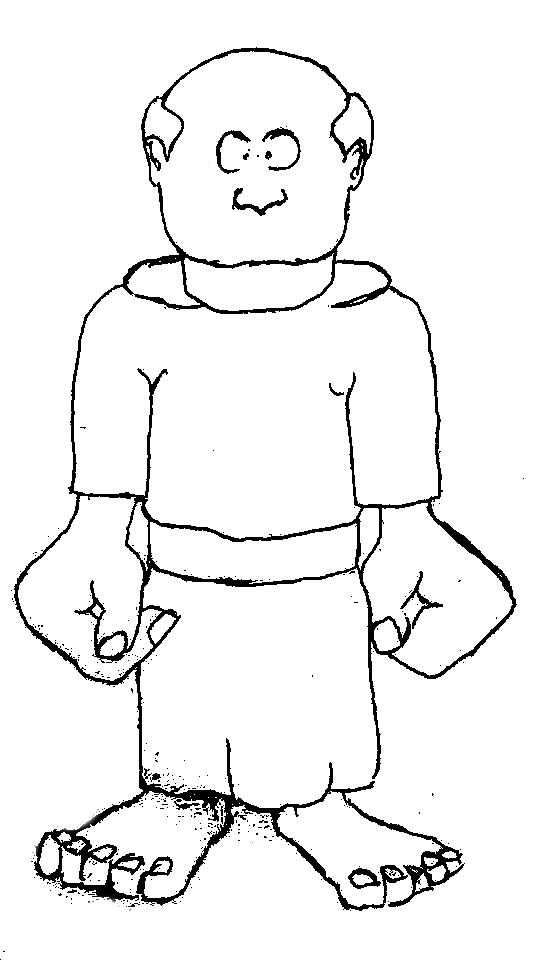
\includegraphics[width=0.7\textwidth]{img/cre-big-hands}	
	\caption{Creationist}
	\label{fig:creationist}
\end{minipage} 
\begin{minipage}[t]{.4\textwidth}
	\centering
	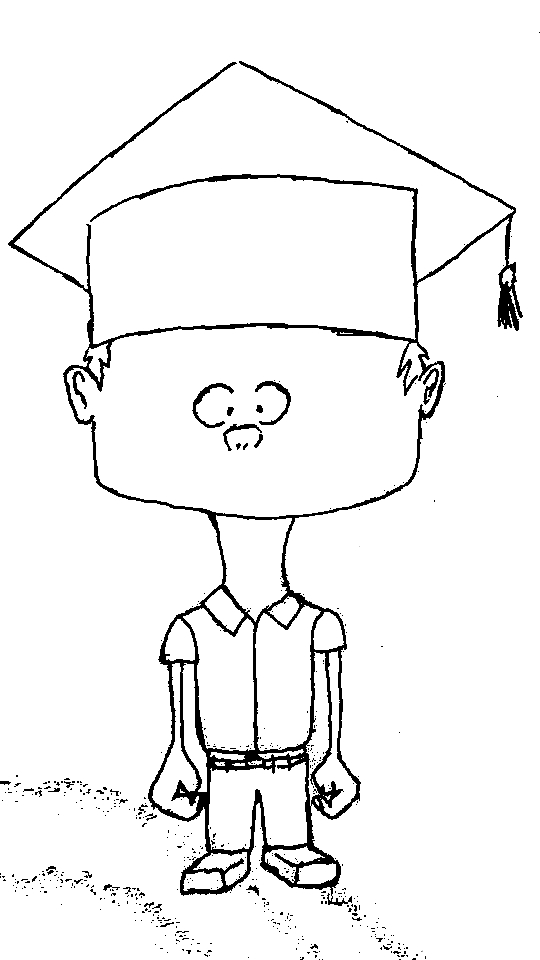
\includegraphics[width=0.7\textwidth]{img/Nerd-BigHead}
	\caption{Scientist}
\end{minipage}
\end{figure}
					
				}
				\subsubsection{Character Upgrades}{
					See table \ref{table:character}
					\begin{table}[h!]\centering
						\begin{tabular}{r!{\color{green2}\vrule}l!{\color{green2}\vrule}l}

							& \textbf{Religious} & \textbf{Evolutionist} \\
							\rowcolor{green1}
							\textit{Immunity against attacks} &	Skin color (white --> silver) & Skin color (white --> silver) \\
							\textit{stronger main Weapon  (upgrade)} &	 Glove color (white --> red) & Gun size (small --> big) \\
							\rowcolor{green1}
							\textit{Faster Running}&	Bigger feet &	Bigger feet  \\
							\textit{Big Wonder skill} & Size of hands (small -->  big)  &	size of head (small --> big)\\
						\end{tabular}
						\caption{\textit{Character Upgrades}}
						\label{table:character}
					\end{table}
						
				}
				
				\subsection{Important Aspects}{
					\begin{enumerate}
						\item \textbf{Fair Teams:}\\
							We want the teams to be equal in the sense that both possess the same offence/defence. Therefore, winning merely depends on the strategy and the aiming skills of the player
						\item \textbf{Unique Gameplay:}\\
							We want our game to be extraordinary, but still playable by common users, without directly fitting into a game category or the need to have long tutorials.
						\item \textbf{Cartoony/Non-Photorealistic Rendering:}\\
							Since we are touching a controversial topic we blind out some seriousness by making the characters and surroundings cartoony
						\item \textbf{Visually stunning and self-explanatory:}\\
							A player should be entertained by simply watching the game. Furthermore it should be self-explanatory without the need of long tutorials
						\item \textbf{Multiple Tasks:}\\
							During the game the player needs to perform different tasks at the same time. On the one hand the game can only be won when a big wonder is cast and thus, players need to form study or praying groups to fill the big wonder bar. On the other hand players must prevent the other team from filling their big wonder bar. Some players in the other team will also pursue this task of distracting the prayers or the studying. Therefore, in order to win the game players also need to protect the players filling the big wonder bar.
					\end{enumerate}

					
					}
		}\label{sec:visual_diff}
	
	}\label{sec:q1sec}
	
	\section{Technical Achievement}
	\label{sec:technicalachievement}
	%to be filled in
	For a game like the one presented in this document the interaction between the players is crucial. Therefore it depends a lot on a rather large group of players, such that the player won't get bored if no one else is around him to interact with. To achieve the player to feel like a part of something big, as well as being attracted by the game by lots of interactions and possibilities to behave is the balance between the level size and the number of players in the game.\\
	
	If the level is very large and there is only a small number of players on the field, everybody is just playing around on his own and not interacting a lot with the other players. It takes a long time to reach the other players to either attack them or to pray or study with them. An experience like this would probably not make the players to fall in love with our game immediately.\\
	
	If, on the other hand, the level is rather small and there are many players on the field, the player will feel challenged and necessary to help his team win the battle. If he has to deal with lots of enemies before being able to reach his fellow campaigners, he will stay active and motivated throughout the entire game. This is the effect we are aiming for.\\
	
	Of course it is not always possible to start a game with that many friends who can join. But since the number of players is really crucial to the game, we will provide non-player characters (\textit{NPC}), which will be controlled by the computer rather than by some human. The artificial intelligence to make these NPCs behave intelligently is the most prominent technical achievement we want to reach. For the player it should not feel different when playing with NPC or with fellow human players. Therefore the artificial intelligence should make the NPC behave similar to characters controlled by humans. On the other hand the artificial intelligence must not be too good. If an NPC is clearly better than the human player, he might feel overchallenged. Therefore we will try to find a good compromise between stupidly behaving NPCs and super-soldier NPC who are invincible.\\
	
	\newpage
	
	
	\section{"Big Idea" Bullseye}
	\label{sec:bigideabullseye}
	\textbf{Big Idea:} Don't Kill, Convert\\
	\textbf{Technical innovation:} Not a standard shooter
	%to be filled in
	
	\begin{figure}[h!]
  		\centering
    	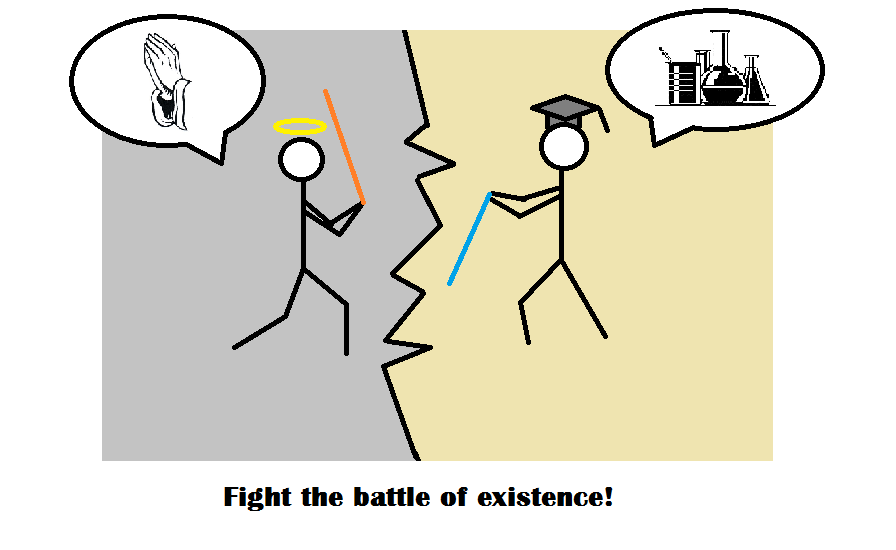
\includegraphics[width=1.0\textwidth]{img/bigideabullseye}
    	\caption{Big idea Bullseye}
	\end{figure}
	
	\section{Development Schedule}{
		\subsection{Layered task breakdown}{
			\begin{enumerate}
				\item Functional Minimum 
					%Minimal items to make something you might call a game 
					\begin{itemize}
						\item Players from two teams running around
						\item Overflow flat Map
						\item Counting collective hits
						\item Game finishes after 8 min
						\item Winner is Team with most hits
						\item AI Controlled Allies/Enemies.
					\end{itemize}
				\item Low target
				%The least possible to feel sort of “ok” about result. 
					\begin{itemize}
						\item Add Audio: Music + Sound Effects
						\item Add Physics:
						\begin{itemize}
							\item Players flying away when hit
							\item Cooldown before being able to move \& attack
							\item Immunity cooldown before being vulnerable again
						\end{itemize}

						\item Add Wonder:
						\begin{itemize}
							\item Wonder is generate after every 50 collective hits
							\item Wonder is possessed by a human player
							\item Wonder can be cast
							\item Wonder visually recognizable			
							\item Wonder converts players
							\item Converted Human player plays for the other team
						\end{itemize}
						\item Winner is the team with the most members
						\item Map includes obstacles
					\end{itemize}
				\item Desired target 
				%This is what you’re aiming for, if things go reasonably well. 
					\begin{itemize}
						\item Characters visually polished to look from same theme
						\item Wonder Creation:
						\begin{itemize}
							\item Creating a wonder by standing together and pressing "commit"
							\item Cooldown after releasing "commit"
							\item Increased vulnerability during praying and cooldown
							\item Larger Praying/Studying Circles will generate quicker progress
							\item AI upgrade to take new wonder creation into account
						\end{itemize}

					\end{itemize}
				\item High target 
				%You might get this much done if things go extremely well. 
					\begin{itemize}
						\item Converted Human player will controls free NPC if available
						\item Evolving Players
						\begin{itemize}
							\item Players evolves numerically according to their actions (Running, Shooting, Praying/Studying)
							\item Players evolves visually
						\end{itemize}
					\end{itemize}
				\item Extras
				%You know won’t fit into this semester, but you might add later. 
					\begin{itemize}
						\item Online multiplayer
						\item Procedural, automatic level-design (each level is different)
						\item Classes of characters (specialized for praying/studying or shooting)		
					\end{itemize}
			\end{enumerate}
		
			
			}
\subsection{Task Allocation}{
	\subsubsection{Project Management}
	See table \ref{table:taskallocProject}
	\subsubsection{Engineering}
	See table \ref{table:taskallocEngineer}
	
	\begin{table}[h!]\centering
		\newcounter{taskId}
		\setcounter{taskId}{0}
		\begin{tabular}{r|p{10cm}|p{1.8cm}|c|c}
			\textbf{Task} & \textbf{Description} & \textbf{Who} & \textbf{Hrs} & \textbf{Actual} \\
			
			\hline 
			\cellcolor[gray]{0.8} & \multicolumn{4}{c}{\cellcolor[gray]{0.8} Idea Finding}\\
			
			\hline						
			\stepcounter{taskId}
			\thetaskId . & Brainstorming Design &\centering  All & $5$ & $7$ \\
			
			\hline
			\stepcounter{taskId}
			\thetaskId . & Character modeling &\centering Gregory  & $20$ & \\
			
			\hline 
			\cellcolor[gray]{0.8} & \multicolumn{4}{c}{\cellcolor[gray]{0.8} Assignments}\\
			
			\hline
			\stepcounter{taskId}
			\thetaskId . & Project Proposal Draft & \centering  All & $10$ & $10$\\
			
			\hline
			\stepcounter{taskId}
			\thetaskId . & Prototype Chapter& \centering  All & $10$ &\\
			
			\hline
			\stepcounter{taskId}
			\thetaskId . & Interim Report Chapter & \centering  All & $10$ &\\
			
			\hline
			\stepcounter{taskId}
			\thetaskId . & Alpha Release Chapter & \centering  All & $10$ &\\
			
			\hline
			\stepcounter{taskId}
			\thetaskId . & Playtest Chapter & \centering  All & $10$ &\\
			
			\hline
			\stepcounter{taskId}
			\thetaskId . & Conclusion Chapter & \centering  All & $10$ &\\
			
			\hline
			\stepcounter{taskId}
			\thetaskId . & Demo Video & \centering Patrick & $50$ &\\
			
			\hline 
			\cellcolor[gray]{0.8} & \multicolumn{4}{c}{\cellcolor[gray]{0.8} Presentation and Demos}\\
			
			\hline
			\stepcounter{taskId}
			\thetaskId . & Pitch of the Game & \centering  All & $7$ & $7$\\
			
			\hline
			\stepcounter{taskId}
			\thetaskId . & Formal Game Proposal & \centering  All & $10$ & $12$\\
			
			\hline
			\stepcounter{taskId}
			\thetaskId . & Paper Prototype & \centering  Jacqueline & $5$ & $6$\\
			
			\hline
			\stepcounter{taskId}
			\thetaskId . & First Playable Demo & \centering  All & $30$ &\\
			
			\hline
			\stepcounter{taskId}
			\thetaskId . & Interim Demo & \centering  All & $50$ &\\
			
			\hline
			\stepcounter{taskId}
			\thetaskId . & Alpha Release Demo & \centering  All & $100$ &\\
			
			\hline
			\stepcounter{taskId}
			\thetaskId . & Play-test presentation & \centering  All & $75$ &\\
			
			\hline
			\stepcounter{taskId}
			\thetaskId . &Final Public Presentation & \centering  All & $40$ &\\
			
		\end{tabular}
		
		\caption{\textit{Task allocation}}
		\label{table:taskallocProject}	
	\end{table}
	
	\begin{table}[h!]\centering
		\begin{tabular}{r|p{10cm}|p{1.8cm}|c|c}
			\textbf{Task} & \textbf{Description} & \textbf{Who} & \textbf{Hrs} & \textbf{Actual} \\
			
			\hline 
			\cellcolor[gray]{0.8} & \multicolumn{4}{c}{\cellcolor[gray]{0.8} Functional Minimum}\\
			
			\hline
			\stepcounter{taskId}
			\thetaskId . & Players from two teams running around & \centering  All & $15$ &\\
			
			\hline
			\stepcounter{taskId}
			\thetaskId . & Level Design: Overflow flat Map & \centering  All & $15$ &\\
			
			
			\hline
			\stepcounter{taskId}
			\thetaskId . & Counting collective hits & \centering  All & $15$ &\\
			
			\hline
			\stepcounter{taskId}
			\thetaskId . & Game finishes after 8 min & \centering  All & $15$ &\\
			
			
			\hline
			\stepcounter{taskId}
			\thetaskId . & Winner is Team with most hits & \centering  All & $15$ &\\
			
			\hline
			\stepcounter{taskId}
			\thetaskId . & AI Controlled Allies/Enemies. & \centering  Ruben & $15$ &\\ 
			
			\hline 
			\cellcolor[gray]{0.8} & \multicolumn{4}{c}{\cellcolor[gray]{0.8} Low Target}\\
			
			\hline
			\stepcounter{taskId}
			\thetaskId . & Audio: Music + Sound Effects & \centering  Patrick & $15$ &\\
			
			\hline
			\stepcounter{taskId}
			\thetaskId . & Physics: Players flying away when hit & \centering  All & $15$ &\\
			
			\hline
			\stepcounter{taskId}
			\thetaskId . & Physics: Cooldown before being able to move \& attack & \centering  All & $15$ &\\
			
			\hline
			\stepcounter{taskId}
			\thetaskId . & Physics: Immunity cooldown before being vulnerable again & \centering  All & $15$ &\\
			
			\hline
			\stepcounter{taskId}
			\thetaskId . & Wonder: Wonder is generate after every 50 collective hits & \centering  All & $15$ &\\
			
			\hline
			\stepcounter{taskId}
			\thetaskId . & Wonder: Wonder is (visually) possessed by a human player & \centering  All & $15$ &\\
			
			\hline
			\stepcounter{taskId}
			\thetaskId . & Wonder: Wonder can visually be cast & \centering  All & $15$ &\\
			
			
			\hline
			\stepcounter{taskId}
			\thetaskId . & Wonder: Wonder converts players & \centering  All & $15$ &\\
			
			\hline
			\stepcounter{taskId}
			\thetaskId . & Wonder: Converted Human player plays for the other team & \centering  All & $15$ &\\
			
			
			\hline
			\stepcounter{taskId}
			\thetaskId . & Winner is the team with the most members & \centering  All & $15$ &\\
			
			\hline
			\stepcounter{taskId}
			\thetaskId . & Level Design: Map includes obstacles & \centering  All & $15$ &\\
			
			\hline 
			\cellcolor[gray]{0.8} & \multicolumn{4}{c}{\cellcolor[gray]{0.8} Desired Target}\\
			\hline
			\stepcounter{taskId}
			\thetaskId . & Characters visually polished to look from same theme & \centering Jacqueline, Gregory & $15$ &\\
			
			\hline
			\stepcounter{taskId}
			\thetaskId . & Wonder Creation: Creating a wonder by standing together and pressing "commit" & \centering  All & $15$ &\\
			
			\hline
			\stepcounter{taskId}
			\thetaskId . & Wonder Creation: Cooldown after releasing "commit" & \centering  All & $15$ &\\
			
			\hline
			\stepcounter{taskId}
			\thetaskId . & Wonder Creation: Increased vulnerability during praying and cooldown & \centering  All & $15$ &\\
			
			\hline
			\stepcounter{taskId}
			\thetaskId . & Wonder Creation: Larger Praying/Studying Circles will generate quicker progress & \centering  All & $15$ &\\
			
			\hline
			\stepcounter{taskId}
			\thetaskId . & Wonder Creation: AI upgrade to take new wonder creation into account & \centering  All & $15$ &\\			
			
			\hline 
			\cellcolor[gray]{0.8} & \multicolumn{4}{c}{\cellcolor[gray]{0.8} High Target}\\
			
			\hline
			\stepcounter{taskId}
			\thetaskId . & Converted Human player will controls free NPC if available & \centering  All & $15$ &\\
			
			\hline
			\stepcounter{taskId}
			\thetaskId . & Players evolves numerically according to their actions (Running, Shooting, Praying/Studying) & \centering  All & $15$ &\\
			
			\hline
			\stepcounter{taskId}
			\thetaskId . & Players evolves visually & \centering  All & $15$ &\\
			
		\end{tabular}
		
		\caption{\textit{Task allocation}}
		\label{table:taskallocEngineer}	
	\end{table}
	 		
}

						\subsection{Timeline}{
				%Detailed timeline, milestones, task accounting, deliverables
				See table \ref{table:timeline}
				
				\begin{table}[h!]\centering
					\setcounter{taskId}{0}
					\begin{tabular}{r|c|c|c|c|c|c|c|c|c|c|c|c|c|c}
						\textbf{Task} & \textbf{W1} & \textbf{W2} & \textbf{W3} & \textbf{W4} & \textbf{W5} & \textbf{W6} & \textbf{W7} & \textbf{W8} & \textbf{W9} & \textbf{W10} & \textbf{W11} & \textbf{W12} & \textbf{W13} & \textbf{W14}\\
						
						\hline 
		\cellcolor[gray]{0.8} & \multicolumn{14}{c}{\cellcolor[gray]{0.8} Idea Finding}\\
						
						\hline						
						\stepcounter{taskId}
						\thetaskId . & A & A & & & & & & & & & & & & \\
						
						\hline						
						\stepcounter{taskId}
						\thetaskId . & G & G & & & & & & & & & & & & \\
						
						\hline 
			\cellcolor[gray]{0.8} & \multicolumn{14}{c}{\cellcolor[gray]{0.8} Assignments}\\
						
						\hline						
						\stepcounter{taskId}
						\thetaskId . & & A & A & & & & & & & & & & & \\
						
						\hline						
						\stepcounter{taskId}
						\thetaskId . & & & & J & A & & & & & & & & & \\
						
						\hline						
						\stepcounter{taskId}
						\thetaskId . & & & & & & A & A & A & A & & & & & \\
						
						\hline						
						\stepcounter{taskId}
						\thetaskId . & & & & & & & & & & A & A & & & \\
						
						\hline						
						\stepcounter{taskId}
						\thetaskId . & & & & & & & & & & & & A & & \\
						
						\hline						
						\stepcounter{taskId}
						\thetaskId . & & & & & & & & & & & & & A & A \\
						
						\hline						
						\stepcounter{taskId}
						\thetaskId . & & & & & & & & & & & & & A & A \\
						
						\hline 
			\cellcolor[gray]{0.8} & \multicolumn{14}{c}{\cellcolor[gray]{0.8} Presentation and Demos}\\
						
						\hline						
						\stepcounter{taskId}
						\thetaskId . & A & & & & & & & & & & & & & \\
						
						\hline						
						\stepcounter{taskId}
						\thetaskId . & & & & A & & & & & & & & & & \\
						
						\hline						
						\stepcounter{taskId}
						\thetaskId . & & & & & & A & & & & & & & & \\
						
						\hline						
						\stepcounter{taskId}
						\thetaskId . & & & & & & & & & A & & & & & \\
						
						\hline						
						\stepcounter{taskId}
						\thetaskId . & & & & & & & & & & & A & & & \\
						
						\hline						
						\stepcounter{taskId}
						\thetaskId . & & & & & & & & & & & & A & & \\
						
						\hline						
						\stepcounter{taskId}
						\thetaskId . & & & & & & & & & & & & & & A \\
						
						\hline						
						\stepcounter{taskId}
						\thetaskId . & & & & & & & & & & & & & & A \\
						
						\hline 
			\cellcolor[gray]{0.8} & \multicolumn{14}{c}{\cellcolor[gray]{0.8} Functional Minimum}\\
						
												\hline						
						\stepcounter{taskId}
						\thetaskId . & & & & & A & & & & & & & & & \\
						
												\hline						
						\stepcounter{taskId}
						\thetaskId . & & & & A & & & & & & & & & & \\
						
												\hline						
						\stepcounter{taskId}
						\thetaskId . & & & & & A & & & & & & & & & \\
						
						\hline 
			\cellcolor[gray]{0.8} & \multicolumn{14}{c}{\cellcolor[gray]{0.8}Low Target}\\
						
						\hline						
						\stepcounter{taskId}
						\thetaskId . & & & & & & P & & & & & & & & \\
						
						\hline						
						\stepcounter{taskId}
						\thetaskId . & & & & & & JG & & & & & & & & \\
						
						\hline						
						\stepcounter{taskId}
						\thetaskId . & & & & & & R & & & & & & & & \\
						
						\hline 
			\cellcolor[gray]{0.8} & \multicolumn{14}{c}{\cellcolor[gray]{0.8} Desired Target}\\
						
						\hline						
						\stepcounter{taskId}
						\thetaskId . & & & & & & & A & & & & & & & \\
						
						\hline						
						\stepcounter{taskId}
						\thetaskId . & & & & & & & A & & & & & & & \\
						
						\hline						
						\stepcounter{taskId}
						\thetaskId . & & & & & & & A & & & & & & & \\
						
						\hline						
						\stepcounter{taskId}
						\thetaskId . & & & & & & & A & & & & & & & \\
						
						\hline						
						\stepcounter{taskId}
						\thetaskId . & & & & & & & & A & & & & & & \\
						
						\hline						
						\stepcounter{taskId}
						\thetaskId . & & & & & & & & A & & & & & & \\
						
						\hline 
			\cellcolor[gray]{0.8} & \multicolumn{14}{c}{\cellcolor[gray]{0.8} High Target}\\
						
						\hline						
						\stepcounter{taskId}
						\thetaskId . & & & & & & & & R & R & & & & & \\
						
						\hline						
						\stepcounter{taskId}
						\thetaskId . & & & & & & & & A & & & & & & \\
						
						\hline						
						\stepcounter{taskId}
						\thetaskId . & & & & & & & & A & A & & & & & \\
								
					\end{tabular}
					
					\caption{\textit{Timeline\\ A = All, P = Patrick, R = Ruben, J = Jacqueline, G = Gregory}}
					\label{table:timeline}
				\end{table} 
				
				
		\section{Assessment}{
			%Strengths, appeal, criteria for success…
			Our game shall stand out in several ways. We want to create a funny, cartoony, visually stunning gaming experience that fascinates someone by only watching another person playing the game. By “funny” we mean that everything from design over physics to sound will be produced with always keeping humour at the back of one’s mind. For example, if a character gets hit by an enemy’s shot, it will fly through the air far away from real-world physics. Also, we want to include a dimension of “cuteness” into our gaming experience by using non-photorealistic rendering and a cartoony overall look. We believe that the combination of cartoony visuals, a camera that shows a wide part of the action and a fast effect-overloaded gameplay will create a special form of appealing that will bring the player in a good mood while providing an experience of fun in every second of playing. By “visually stunning” we want to say that the player will see a battlefield with a lot of characters fighting each other and building pray/study circles, objects that are hit and therefore flying through the air, different looking characters according to their skills and a lot of light and particle effects caused by the weapons, power-ups or the skills of characters.
			As criteria for success we elaborated our own “big idea bullseye”. On the one hand, our core idea consists of the effect-overloaded non-realistic cartoony styled fight over evolution including the “super-power” of converting enemies. On the other hand, our technical innovation is a shooter where you can’t kill enemies and where team play is crucial to win the game.
			
		}
	}	
	
\end{document}}{den}